%!TEX root = ../../thesis.tex
%!TEX enableSynctex = true
%*******************************************************************************
%*********************************** First Chapter *****************************
%*******************************************************************************

\ifpdf
    \graphicspath{{Chapters/principles/Figs/Raster/}{Chapters/principles/Figs/PDF/}{Chapters/principles/Figs/}}
\else
    \graphicspath{{Chapters/principles/Figs/Vector/}{Chapters/principles/Figs/}}
\fi

\chapter{Principles of fluorescence microscopy}\label{chapter:principles}
% \epigraph{\emph{3D Airy disk renderings: \(E \) there or \(E^2 \)}}{--- Roxine Staats}
%Physical prciniples of the operation of a light-microscope.
%Capabilities limtiations.

This chapter introduces the concept of the light microscope in contemporary fluorescence microscopy.
Basic geometrical optics and properties of light waves are presented to understand the construction and functioning of light microscopes and light-sheet microscopes in particular.
The concepts presented here will be elementary and recalled in later chapters.

% Light sources and detectors are discussed focusing on read-out methods from detectors which has become important in many types of microscopy but notably light sheet microscopy due to the high frame rates required and the contrast enhancement from confocal slit scanning.
%
% Finally an overview of 3D microscopy methods is provided including detailed discussion of 3D SIm the principle of which can be applied in light sheet microscopy as discussed in chapter <xx>

\pagebreak
\section{Light microscopy}
% The simplest lens set of an objective collecting lens (close to the sample) and a tube lens (for relaying the image), drives the imaging of most modern microscopes.

\subsection{Construction of light microscopes}

%Consists of illumination elements and detection elements.

% \subsubsection{Components of light microscopes}
%Imaging part of microscope is formed of two leneses
%Infinity corrected system.
The fundamental concept of a light microscope requires a set of lenses to relay and magnify the image of a remote object or specimen using light as a measurand.
% The key driver of the imaging aspect of an optical microscope is a pair of lenses.
The sample is located in the front focal plane of the \emph{\gls{objective lens}} and the resultant image is focused onto the \emph{\gls{primary imaging plane}}, see \figurename~\ref{fig:magnification}.
Light emitted by a point \(o_1 \) at the sample plane is transformed into a parallel ray bundle by the \gls{objective lens}, which travels parallel to the optical axis.
The tube lens then refracts the ray bundle back down onto its focus.
The ray bundle for a point away \(o_2 \) from the optical axis can be determined by the \emph{chief ray} (\(r_c \)) which passes through the optical centre of the objective unperturbed, and the \emph{marginal ray} (\(r_m \)) travelling parallel to the optical axis which crosses the back-focal point of the \gls{objective lens}.
Both of these rays propagate in parallel within the \emph{infinity space} between the objective and tube lens, as do all sets of rays at any point \(o_n \) at the focal plane of the \gls{objective lens}.

\subsubsection{Magnification}
\index{magnification}
\index{ray optics}

Due to the parallel propagation of rays in the infinity space the distance between the two lenses may be selected arbitrarily.
Typically the back focal points are matched to create a \emph{\gls{4f} system}, as shown in \figurename~\ref{fig:magnification}, as this configuration improves imaging quality by reducing optical aberrations.

The marginal (\(r_m' \)) and chief (\(r_c' \)) rays incident on the tube lens then govern where a real image of the sample lies at the \emph{primary image plane}.
\(o_1' \)
The image size (\(O' \)) in the primary image plane is set by the distance between the intersection of the primary image plane to the intersect of the the margin (\(r_m' \)) and chief rays (\(r_c' \)) at the tube lens.
% The marginal rays for each lens in a \gls{4f} system will

% \gls{alpha}

\begin{align}
    \tan \gls{alpha} &= \frac{O}{f_{\text{objective}}} =  \frac{O'}{f_{\text{tube lens}}} \\
    \intertext{It follows that the lateral magnification of the sample is:}
    \implies M &= \frac{O'}{O} = \frac{f_{\text{tube lens}}}
{f_{\text{objective}}}
\end{align}

\begin{figure}
    \centering
    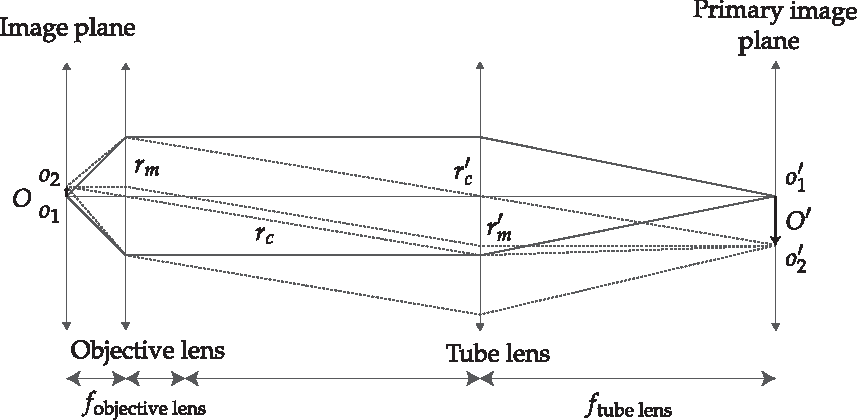
\includegraphics{./magnification}
    \caption{Ray diagram of a two lens magnification system, with a \gls{4f} configuration.}
    \label{fig:magnification}
\end{figure}

% Tube lens may also be used to correct for image abberations

%Great advantage is that the lgiht path behind the objective only contains paralel light, means can add optical elements without distortions the beam path.

% Other adsvantage is you can focus by moving the \gls{objective lens}

%and the overall magnification of the

%\subsubsection{Magnification}

\subsubsection{Field of view}

\index{field of view}

The observable objective \gls{FOV} is limited by the aperture stop of the system typified as the field number (\(F_\text{n}  \)) and the \gls{objective lens} magnification \(M_{\text{objective}} \):
%The maximum field of view (\(F_{n} \))available is by :

\begin{align}
    \gls{FOV} = \frac{F_{n}}{M_{\text{objective}}}
\end{align}

The field number achievable in a real \gls{objective lens} design is limited by the image degradation caused through optical aberrations.
Modern objective technology can reach up to \SI{28}{\milli\meter} from the previous standard of \SI{20}{\milli\meter}.

\subsubsection{Illumination}

The illumination system defines the contrast mode, the resolution of the instrument, and the overall brightness.
Two principally different optical setups are in use in optical microscopes.
The optically simpler of the two is the source focus or critical illumination and the other, which is by far more prevalent, is called Köhler illumination.

Critical illumination uses a single \emph{condenser} lens whereas Kohler illumination uses an additional \emph{collector} lens.
The use of two illumination lenses allows for a conjugate \gls{4f}  system of illumination to the detection optics, this ensures that all ray bundles passing through the sample are parallel and the illumination brightness is homogenous.
Having a conjugated illumination also allows for alternative contrast methods to be implemented.

In the illumination beam paths discussed earlier, the specimen is placed between the light source and the \gls{objective lens}.
In many cases, however, it is advantageous to illuminate the specimen from the side of observation (\emph{epi-illumnination}).
For instance, when looking at the reflection of opaque samples, or the emission of fluorescent samples.
Optically the illumination is the same or similar with the condenser lens then being the imaging \gls{objective lens} as well.
% In that case, some optical components of illumination and imaging are identical, for example, the \gls{objective lens}.

\subsection{Resolution}\label{sec:resolution}\index{resolution}
%Magification versus resolution

Resolution refers to the fineness of detail that can be recognised in an image, such as small and intricate structures or the distance between closely placed small objects.
The latter case, specifically the smallest separation at which two point-like emitters produce an image that can be distinguished as coming from two sources, is used to define and quantify the optical resolution.
% Using light microscopy
% Using light microscopy, minute objects can be discriminated from each other when they are positioned at a minimum distance of -0.25 mum from each other and green light and a high-quality oil-immersion \gls{objective lens} are used.
% This obviously means that proteins and supramolecular complexes occurring in living cells cannot be recognized in detail.
% In later chapters, we discuss how the principal optical resolution limit can be overcome or circumvented by advanced optical techniques.

\subsubsection{Angular aperture and numerical aperture}\index{numerical aperture}

%An \gls{objective lens}es is limited by
The maximum half acceptance angle (\gls{alpha}) of an \gls{objective lens} limits the amount of light that can be collected from the sample.
It is the half angle of the cone at the optical centre of the objective lens, outside of which light is not collected for imaging.
An \gls{objective lens} may be approximated to applying a Fourier transform of the imaging space, through an aperture with radius \(a\) with an imaging plane at the far field.
This leads to high frequency information being omitted during the imaging process and the lens behaving as a low-pass filter for optical frequencies.
The electric field (\gls{E}\((r)\)) and resultant intensity (\gls{I}\((r)\)) distribution of a single point (delta function) at the primary image plane then becomes:

\begin{align}
    E(r) &\propto E_0 \frac{J_1 \left( \frac{2\pi r}{\lambda}\sin \alpha \right)}{ \frac{2\pi r}{\lambda} \sin {\alpha})}\label{eq:E_airy}\\
    \implies
    I(r) &= I_0 \left[\frac{J_1 \left( \frac{2\pi r}{\lambda} \sin \alpha \right)}{ \frac{2\pi r}{\lambda} \sin {\alpha})}\right]^2\label{eq:I_airy}
\end{align}

Where \gls{J_1} is a Bessel function of the first kind and \gls{alpha} is the half opening angle of the objective lens.
This function is more commonly known as an \Gls{airy disk} as shown in \figurename~\ref{fig:airy_disk}.

\begin{figure}
    \centering
    \begin{subfigure}[b]{\textwidth}
        %\centering
        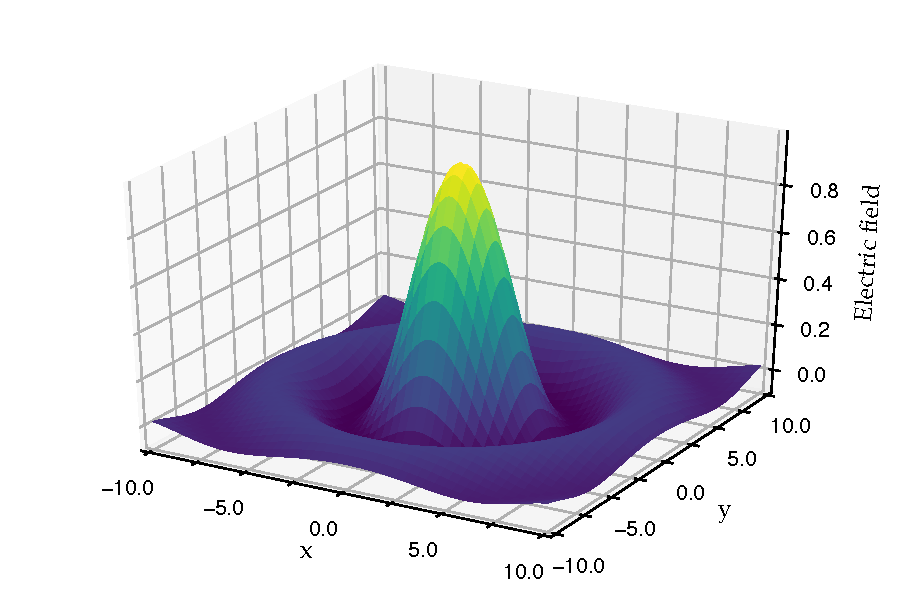
\includegraphics{+airy_E_fill}
        \caption{\(E(r)\), equation~\eqref{eq:E_airy}}\label{fig:airy_E_fill}
    \end{subfigure}\quad
    \begin{subfigure}[b]{\textwidth}
        %\centering
        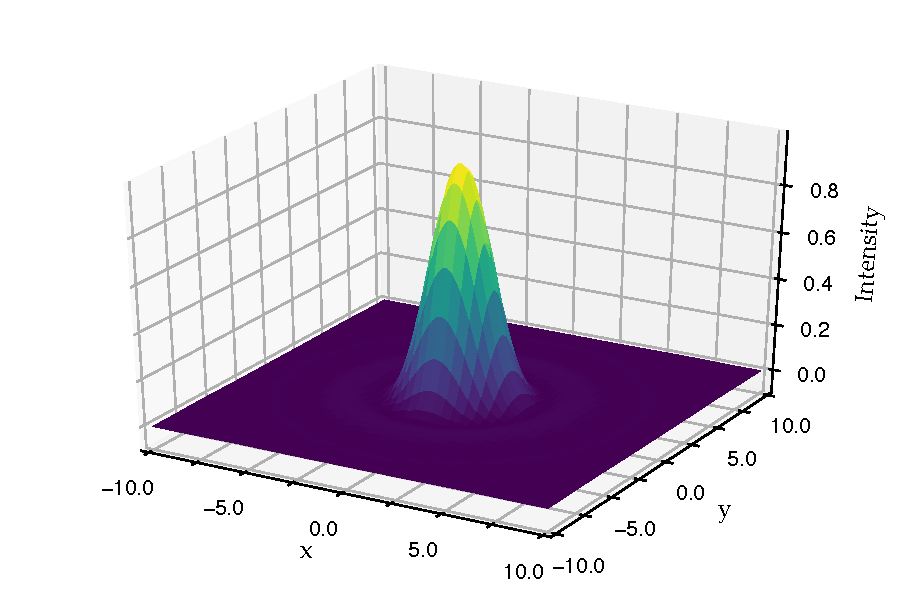
\includegraphics{+airy_I_fill}
        \caption{\(I(r)\), equation~\eqref{eq:I_airy}}\label{fig:airy_I_fill}
    \end{subfigure}
    \caption[Electric and intensity amplitudes of a theoretical \gls{airy disk}]{Electric and intensity amplitudes of a theoretical \gls{airy disk}, lateral distances \(x\) and \(y\) are given in units of \(\frac{2\pi r }{\lambda}\sin {\alpha}\)}\label{fig:airy_disk}
\end{figure}

\subsubsection{Lateral resolution}

Point emitters are therefore imaged more faithfully with wider collecting angles and with shorter wavelength light.
By placing two point emitters close such that the first zero crossing of the Bessel function \gls{J_1} coincides with the centre of the second point emitter gives a distance of:

\begin{align}
    r_{0,\text{objective}} &\approx \frac{0.61\lambda}{n\sin\alpha} = d_r \label{eq:lateral_res}\\
    \implies d_r &= \frac{1.22 \lambda}{NA_{\text{objective}}}
\end{align}

The resulting distance is Rayleigh's criterion for resolution which provides a limit to the resolution of a system based on a dip in intensity maxima, between two neighbouring emitters, of \SI{75}{\percent} as shown in \figurename~\ref{fig:airy_rayleigh}.

%Coherent and incoherent
\subsubsection{Axial resolution}

The \Gls{airy disk} describes the in-plane lateral intensity distribution, with an analogous analytical function propagating axially.
Once again, by comparing the the distance to the first zero in intensity along \(z\) an analytical definition can be formed:

\begin{align}
    z_{0,\text{objective}} = \frac{2n\lambda}{{NA}^2} \label{eq:axial_res} = \frac{1}{2} D_{\text{objective}}
\end{align}

The achievable axial resolution is governed by axial extension of the \gls{PSF} which is \(2z_{0,\text{objective}}\) and is commonly called the \emph{\gls{depth of field}} (\(D_{\text{objective}}\)).
The \gls{depth of field} physically refers to the distance a focussed object may be moved axially before losing image fidelity to defocus.

\begin{figure}
    \centering
    \begin{subfigure}[b]{\textwidth}
        \centering
        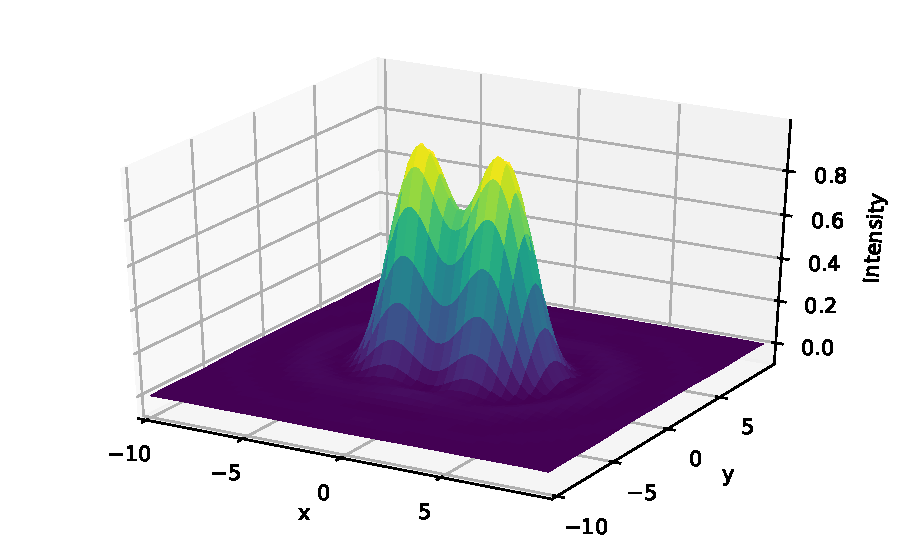
\includegraphics{+airy_rayleigh}
        \caption{The Rayleigh criteon, whereby the centre of the second emitter sits at the first zero of the first emitter.}\label{fig:airy_rayleigh}
    \end{subfigure}
    \begin{subfigure}[b]{\textwidth}
        %\centering
        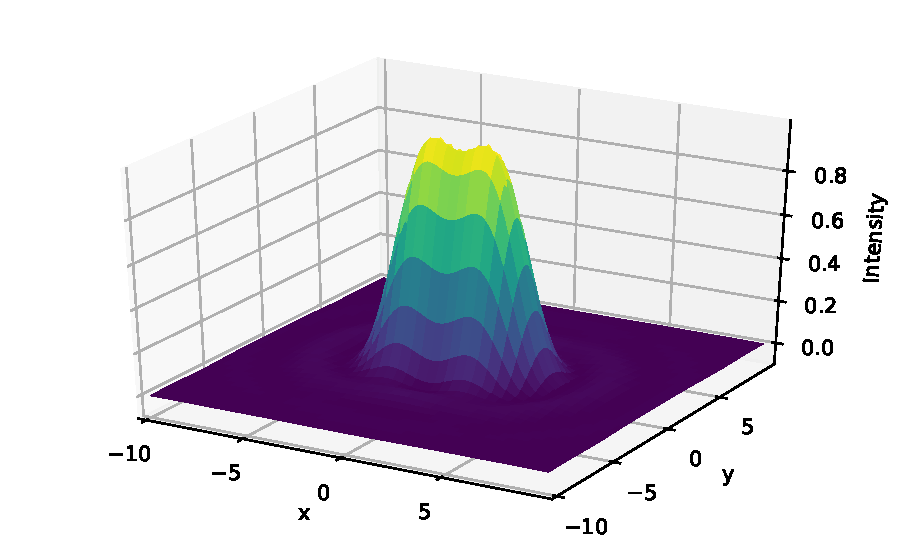
\includegraphics{+airy_sparrow}
        \caption{The Sparrow criteon, whereby the centre of the second emitter is one \gls{FWHM} of the function distant from the first emitter.}\label{fig:airy_sparrow}
    \end{subfigure}
    \end{figure}
    \begin{figure}
\ContinuedFloat\begin{subfigure}[b]{\textwidth}
        %\centering
        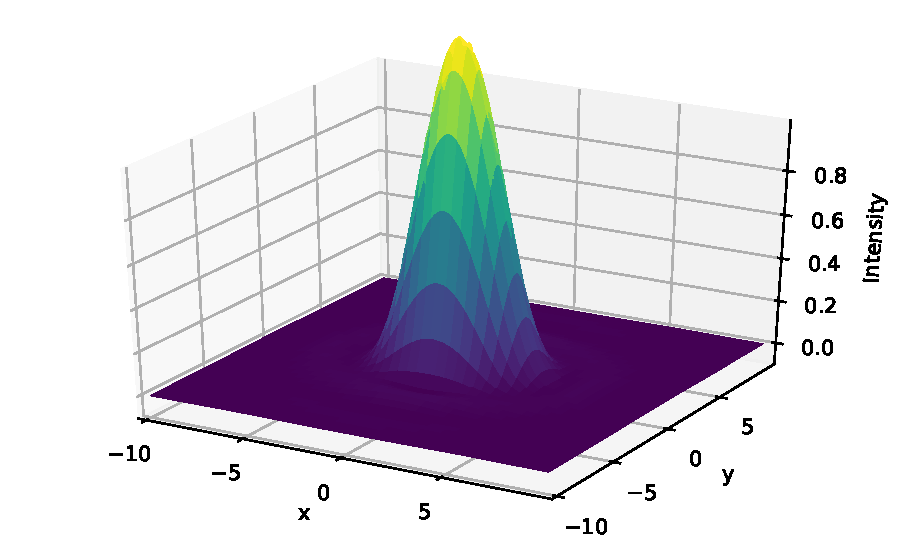
\includegraphics{+airy_too_close}
        \caption{Unresolved, depicted here as being half the Sparrow limit}\label{fig:airy_too_close}
    \end{subfigure}
    \caption[Resolution criterion]{The resolution of a system is governed by the resolving capability of two nearby point emitters.
    (\subref{fig:airy_rayleigh}) and (\subref{fig:airy_sparrow}) show the Rayleigh and Sparrow criterions respectively with (\subref{fig:airy_too_close}) showing point emitters too near to be resolved due to the lack of any intensity contrast between them}\label{fig:airy_disk_resolution}.
\end{figure}

% Depth of field
%
% \subsubsection{Depth of field}

\subsubsection{Sampling}

% \index{Nyquist sampling}

Once transmitted, the irradiance image produced in the primary image plane is typically recorded digitally, using using a \gls{CCD} array sensor or similar device (e.g.~an \gls{sCMOS} array).
According to \Gls{nyquist sampling theory}, the resolution of the detector (i.e.~the pitch separating the adjacent rows of sensor elements, \gls{photosite}s) required to resample the image information faithfully is \(d_\text{detector} = \frac{d_r}{2}\).
To then choose the correct system magnification (\(M_\text{system}\)) it follows that:

\begin{align}
    M_\text{system} = \frac{2d_\text{detector}}{d_r}
\end{align}

For a detector with \gls{photosite}s (detector pixels) in a square array with a pitch of \SI{6}{\micro\meter}, a magnification on the order of \(50\times \) is sufficient for diffraction limited imaging using visible light.\index{magnification}
Magnification in excess of this limit is deemed \emph{empty magnification} and decreases the overall \gls{SNR} of the recorded image.
However, such over-sampling plays an important role in super-resolved systems where the additional pixel information, though diffraction limited, may be used to increase resolution computationally~\cite{betzigImagingIntracellularFluorescent2006}.
\pagebreak
\begin{figure}
    \centering
    \begin{subfigure}[b]{\textwidth}
        \centering
        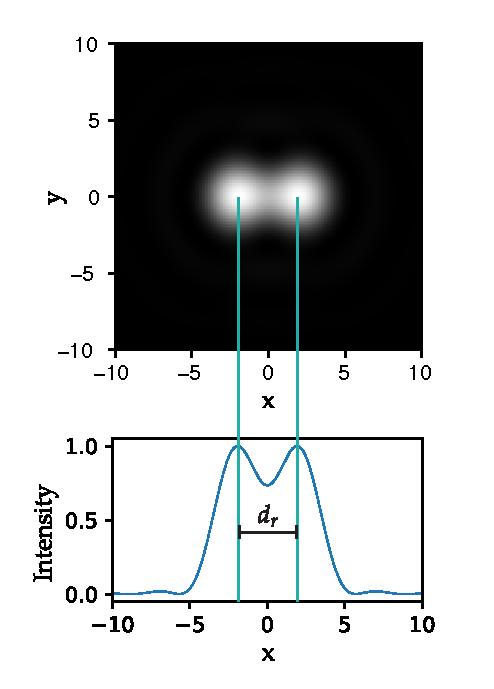
\includegraphics{./sampling/sample_master}
        \caption{Intensity image of a pair of resolved point emitters separated by the Rayleigh distance \(d_{r} \), where \(x \) is lateral distance in units of \(\frac{2\pi r }{\lambda}\sin {\alpha} \) and intensity quantifies irradiance (\SI{}{\watt\per\meter\square} in the primary image plane.)}\label{fig:sample_master}
    \end{subfigure}
\end{figure}
\begin{figure}
\ContinuedFloat\centering
      \begin{subfigure}[t]{0.4\textwidth}
        \centering
        
\includegraphics[width=0.9\textwidth]{./sampling/digital_airy_sample_3}
        \caption{Sampled using 3 by 3 pixels\\
        \(d_{\text{detector}} = 1.5 \times d_{r}M_{\text{system}}\)}\label{fig:digital_airy_sample_3}
    \end{subfigure}\quad
    \begin{subfigure}[t]{0.4\textwidth}
        \centering
        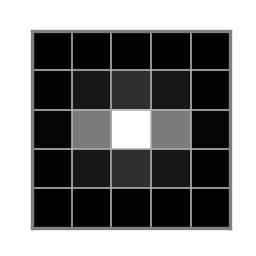
\includegraphics[width=0.9\textwidth]{./sampling/digital_airy_sample_5}
        \caption{Sampled using 5 by 5 pixels\\
        \(d_{\text{detector}} = 0.9 \times  d_{r}M_{\text{system}}\)}\label{fig:digital_airy_sample_5}
    \end{subfigure}\\
    \begin{subfigure}[t]{0.4\textwidth}
        \centering
        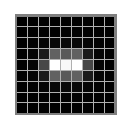
\includegraphics[width=0.9\textwidth]{./sampling/digital_airy_sample_9}
        \caption{Sampled using 9 by 9 pixels\\
        \(d_{\text{detector}} = 0.5 \times d_{r}M_{\text{system}}\)}\label{fig:digital_airy_sample_9}
    \end{subfigure}\quad
    \begin{subfigure}[t]{0.4\textwidth}
        \centering
        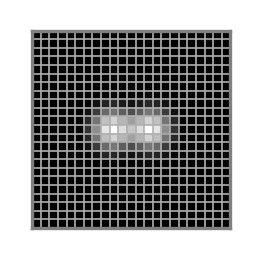
\includegraphics[width=0.9\textwidth]{./sampling/digital_airy_sample_23}
        \caption{Sampled using 23 by 23 pixels\\
        \(d_{\text{detector}} = 0.19 \times d_{r}M_{\text{system}}\)}\label{fig:digital_airy_sample_23}
    \end{subfigure}\\
    \begin{subfigure}[t]{\textwidth}
      \vspace{\abovecaptionskip}
      \centering
      
\includegraphics{./sampling/colourbar}\\
      Irradiance in primary image plane
    \end{subfigure}
    % \begin{subfigure}[t]{0.1\textwidth}
    %     \centering
    %     
\includegraphics{./sampling/colourbar}
    %     % \caption{Sampled using 23 by 23 pixels\\\(d_{\text{detector}} = 0.19 \times d_{r}M_{\text{system}}\)}
    %     % \label{fig:digital_airy_sample_23}
    % \end{subfigure}
    \caption[The effect of sampling on a \gls{PSF}]{The effect of sampling on a \gls{PSF}.
    Point emitters in (\subref{fig:sample_master}) are sampled by a detector with varying detector pixel widths relative to the optical resolution of the system.
    % analogous to varying magnification.
    (\subref{fig:digital_airy_sample_9}), shows Nyquist sampling;
    (\subref{fig:digital_airy_sample_23}) is over sampled, giving super detector resolution.
    (\subref{fig:digital_airy_sample_3}) and (\subref{fig:digital_airy_sample_5}) do not preserve resolution as they are below Nyquist sampling and the images may be mis-interpretted as being produced by a single emitter or by a continuous feature, instead of two distinct point emitters and hence detect a single emitter.}\label{fig:digital_airy}
\end{figure}
\pagebreak

% \subsubsection{Light collection efficiency}
%
% To calculate the the collecting efficiency of a lens, a single radiating source is considered, a Lambert radiator.
% The flux collected is proportional to the spherical segment carved out by the lens.


\section{Fluorescence microscopy}
\subsection{Contrast in optical microscopy}
% Phase contrast, dark field
\subsection{Fluorescence}\index{fluorescence}

Fluorescent molecules absorb photons of a particular energy with an excitation wavelength (\(\lambda \)) (where energy \(= h \nu = h \frac{c}{\lambda}\)), a short time later the molecules re-emit a photon with lower energy, this energy difference gives rise to a red-shift of the emitted photon.
This shift in colour allows for suitably coated glass to chromatically separate the desired fluorescent signal and the undesired scattered incident light.
% Upon being exciting by incident light, an electron within a fluorescent molecule may excite to a higher energy level, provided it has sufficient potential energy to traverse the energy barrier.
Upon being exciting by incident light, a fluorescent species may be transformed to a higher level state.
The occurs when an electron in the ground state energy level absorbs an incident photon with an energy greater than the difference of the exited state (\(S_1\)) and the ground state (\(S_0\))
Once in the higher excited state (\(S_1\)), \gls{fluorophore}s will exist there for an average lifetime (\gls{tau}), slowly losing energy to the surroundings through vibrations and molecular collisions.
Once the electron has \emph{trickled} down the energy levels, it will return to the ground state (\(S_0 \)) emitting a photon with an energy less the amount of energy lost when in the excited state, the \emph{\Gls{stokes shift}}.
Electrons may also return to the ground state through molecular collisions or an \emph{intersystem} crossing whereby the electron finds a path via transient states with lower energy requirements, such as the \emph{triplet state}, shown in \figurename~\ref{fig:jablonski_triplet_new}

%\subsubsection{Fluoresence spectra}
In practice, multiple (split) energy levels slightly above the ground and excited states tend to promote a distribution of multiple different emission wavelengths.
Fluorescent molecules therefore have broad excitation and emission spectra rather than discrete excitation and emission lines, see \figurename~\ref{fig:fluo_spectra} for typical fluorescent molecules used in microscopy.

An important advantage of fluorescence microscopy is labelling \emph{\gls{specificity}}, which refers to the ability to accurately label markers, features or molecules within a specimen.
Multiple labels in different spectral windows can further elucidate how labelled entities interact within the sample.

\begin{figure}
    \centering
    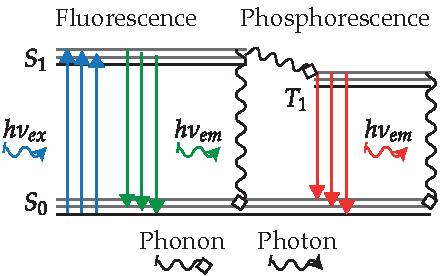
\includegraphics{jablonski_triplet_newer}
    \caption[Standard jablonski diagram]{
    Jablonski diagram representing a green fluorescent molecule.
    Transitions are indicated as excitation (\emph{ex}) or emission (\emph{em}). %represented by waving vectors.
    Species in state \(S_0 \) receive energy from blue incident light,
    this causes the electrons to transition to state \(S_1 \).
    From \(S_1 \) species may lose energy non-radiatively and re-emit a greener photon when relaxing back to \(S_0 \).
    Once in \(S_1 \) electrons may transition to a triplet state, re-emitting a photon through phosphorescence.
    A molecule in a triplet state will be for a longer time to \(S_1 \) and with an increased chance of oxidation which causes photobleaching.%risk photobleaching through oxidation
    }\label{fig:jablonski_triplet_new}
\end{figure}
%\subsubsection{Specificity}


\subsubsection{Labelling}\index{labelling}

% Labelling of sites direct, primary and secondary.
Fluorescent labels may be attached to a site on a molecule directly, using primary antibodies or secondary antibodies.
Direct immunolabeling involves attaching an antibody to the target molecule directly and having the dye molecule attach to another site on the antibody.
Indirect immunolabeling labelling attaches a secondary antibody to the primary antibody and attaches a fluorescent dye to the secondary.
Indirect immunolabeling labelling has the advantage of ease of labelling for most target molecules with most dye molecules.
However, effective resolution (which is distinct from imaging resolution in that effective resolution refers to locating target species) is lost due to the longer ligand attaching to the target.%, but for convenience of dyes with the suitable anti-group being available.
% Ligand length is also dependant of the type of staining, direct or secondary.
% Direct labels refer to the dye directly binding to an active site on the molecule of interest,
The staining process is further inhibited by cellular mechanics; a cell may not take up (endocytose) the stain or be it may degraded by the cell (through \gls{autophagy} in the \gls{lysosome}).

For non-membrane permeable dyes, \gls{transfection} techniques, though invasive, do exist~\cite{kimMammalianCellTransfection2010}.
Staining can also lead to non-specific binding of fluorescent molecules reducing confidence in specificity and increasing the overall background fluorescent signal in-turn decreasing the image contrast.

For live organism imaging, staining is impractical.
Genetic manipulation can allow for fluorescent proteins to be expressed with high specificity as the cells themselves are producing the desired \gls{fluorophore}, covalently bonded to the target molecule; with good spatial homogeneity when compared to soaking samples in dye; and low sample toxicity.

%TODO Talk about auto Fluoresence

%NC :

% Can you put a brief section here on filter sets? This wopuld make your jump from talking about lasers to detectors less jarring.
%
% I think you also need a short paragraph summarising what people usually do (most people use lasers for point scanning and super res due to the high intensity for multiple colour microscopy people usually combine lasers these wavelength are most comon. NThen talk about spectral selection.
%
% Lasers are combined using dichroic mirrors then snt to the sample a dichroic seperates the excitation and emission into different paths and emission filters further suppres out of band signal. An example excitation laser and filter set for 3 colour imaging is shown in figure..

%\subsubsection{Image contrast}
%\subsubsection{Specificity}
\subsection{Fluoresence microscopy}

\subsubsection{Illumnination}

%The Merucry Arc lamp is unibiqitous in lamp-based fluorsence mciroscopes.
The mercury arc lamp became the ubiquitous excitation source for fluorescence microscopy because it emits a broad visible emission spectrum at a higher intensity than a standard halogen lamp.
However, advances in \gls{LED} and \gls{Laser} technology have caused a technological shift towards these alternative sources especially in fluroesence microscopy where narrow spectrum excitation light sources are desirable.
Modern \gls{LED}s and \gls{Laser}s are now have the the stability and intensity to compete with lamp based sources, with more available intensity and homogeneity.

\gls{LED} sources are currently behind Lasers in terms of the intensity required for certain imaging applications due to the \emph{\gls{etendue}} (or geometric extent defined as the product solid angle of of the system's entrance pupil and the area which is conserved through optical systems) of the emission.
As \gls{etendue} is preserved through any system of optics an \gls{LED} source, having large \gls{etendue}, will be very photon inefficient, to the point of being infeasible for applications such as point-scanning.

\Gls{Laser}s are generally limited to very specific excitation lines due to the materials used, particularly in the case of diode lasers.
\Gls{Laser} light sources are also optically \gls{coherent} which causes self-interference in the illumination profile (speckle) and the sample.
%For wide-field imaging LED sources may be sufficient with an added benefit of being incoherent.
%Emission wavelengths are selected from lamp and white LED sources using emission filters.
A \gls{super-continuum laser} sources uses non-linear optical effects, typically induced within a long photonic crystal fibre, to produce broad-spectrum visible \gls{Laser} light.
From this spectrum, wavelengths may then be selected using emission filters, as with lamp-based sources and white LED sources.
This is in contrast to systems with monochromatic lasers as adding more laser lines requires the physical addition of a new laser, making \gls{super-continuum laser}s versatile.
% The downside being that t
However, the intensity of the of the pump laser source is spread into the entire spectrum causing narrow selected emission bands to have relatively low intensities.
% To add additional emission lines into a system with monochromatic lasers requires adding more laser lines physically, this approach is desirable for making systems versatile.
% The downside being that the intensity of the of the pump laser source is spread into the entire spectrum causing narrow selected emission bands to have relatively low intensities.

\begin{figure}
    \centering
    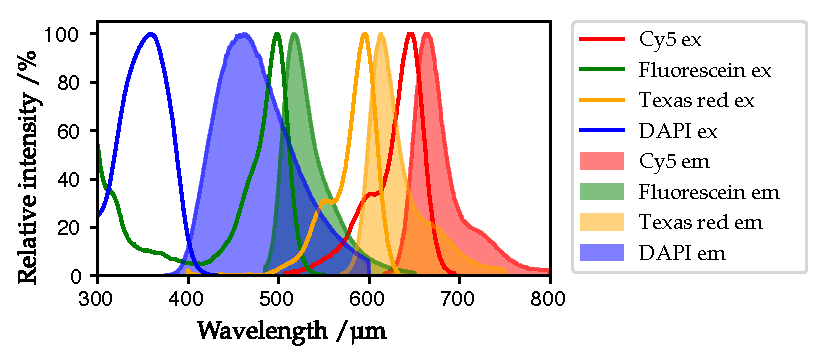
\includegraphics{./fluorphores/++multi_plot.pdf}
    \caption[Common fluorescence excitation spectra]{Fluorescence excitation (lines) and emission (filled curves) spectra of the compounds Fluorescein, Texas red, Cy5 (all homocyclic) and DAPI.}\label{fig:fluo_spectra}\index{fluorescence spectra}
\end{figure}

\subsection{Signal collection}

Once created, the detected image is recorded for analysis and dissemination.
%Modern camera technology
Sensors made up of digital \gls{pixel} (\gls{photosite}) arrays are used in \gls{wide-field} fluoresce microscopes (e.g. \gls{CMOS} and \gls{CCD}) and photo-multiplier tubes (PMT) are used in most laser scanning microscopy.

\subsubsection{Detectors}\index{detectors}

Modern \gls{wide-field} detectors come in many types, all of which exploit semi-conductor physics to convert incident photons into electrons.
\Gls{CCD} based detectors collect electrons during an exposure and transfer in a serial manner through conversion electronics to create digital images, as depicted in \figurename~\ref{fig:sensor_chips}.
\Gls{ICCD} detectors follow the same protocol but use on-photo-site electron cascading to increase the signal and \emph{intensify} the read image.
\gls{EMCCD} detectors transfer their entire frame to a separate conjugate chip which digitises the image for computation.
As the frame is being transferred the signal is amplified to multiply electrons collected in the conjugate digitisation site and intensify the image as in \gls{ICCD}.
Transferring the entire frame reduces the digitalisation time and increase the imaging frame-rate.

\gls{CMOS} chips directly convert radiant exposure to a digital value on a per pixel basis.
The additional circuity found off-chip in \gls{CCD} detectors is embedded in each pixel.
Though this reduces the overall fill factor feasible in each chip, this can be recovered using a micro-lens array to focus directly onto the active read area of the \gls{photosite}.
The per-photo-site architecture allows for a region-of-interest area to be addressed.
\gls{CMOS} detectors made specifically to address quantitative scientific (\gls{sCMOS}) usage tend to have: small pixel sizes; low read noise; large detection arrays; large dynamic range and no multiplicative noise~\cite{verveerAdvancedFluorescenceMicroscopy2015}.

%\subsubsection{Single molecule detection}

\subsubsection{Sensor model}

Each measured pixel value in the digital image, \(y_i\), is therefore modelled as follows, where \(t_\text{exp}\) is the exposure time, \(g\) is the gain, \(a_i\) a per-pixel factor to allow for non-uniform response to illumination (often assumed constant is unity) and \(f_i\) the incident radiant flux on the photo-site. The numbers of the photo-electronics collected at the photo-site is Poisson-distributed, with expected value:
\begin{align}
  E(e_i) = t_\text{exp} a_i f_i
  \intertext{The recorded pixel value is affect by sensor gain and fixed readout noise:}
  y_i = g(a_i) + r_i(g)
  \intertext{\(f_i\) (irradiance) can be quantified from \(\mathbf{y}\) by taking a bias frame \(\mathbf{b}\) and estimate:}
  \hat{f_i} = \frac{y_i-b_i}{g t_\text{exp} a_i}
\end{align}

\subsubsection{Noise}\index{detector noise}

Adverse noise arises in optical microscopes from several compounding effects.
The larger the noise level the lower the \gls{SNR} and the more degraded the recorded image will be.

The \emph{\gls{dark current}} (noise) contribution occurs in the detectors themselves as the semiconductor material produces erroneous electrons from converting thermal phonons.
\Gls{dark current} increases linearly with integration time and so chip cooling is recommended.
\emph{\Gls{photon noise}} (shot) originates from corpuscular photons arriving at the detector following a temporal \Gls{poissonian distribution}.
An image containing \(n \) photons will suffer a variation of \(\sqrt{n} \) in photons being emitted, this can appear as valid structure once recorded.
\emph{\Gls{read noise}} is rooted in the conversion process of the analogue voltage of electrons, at each \gls{pixel}, to digital values.
The intensity response across a detector may also be inhomogeneous, this may be flat-field corrected using a calibration from a uniform intensity source.
\footnote{manufacturers for \gls{sCMOS} cameras apply this correction as standard}

A detector with a large \emph{\gls{quantum efficiency}} (photon to electron conversion efficiency), will be able to overcome noise more quickly.
The \emph{\gls{dynamic range}} of the detector is the intensity range at which the weak fluorescent signal can be recorded above background noise.
The \emph{\gls{bit depth}} (8 or \SI{16}{\bit} typically) of the detector defines the detectable intensity resolution, which is of particular use for very weak signals.
Increasing the integration (exposure) time of the detector will bring the desired signal out of random background noise.
However this can be limited by other effects such as sample movement on the timescale of imaging or photobleaching.
%NC
%Close with noise is one factor which limits fluorescence microscopy.
% One way of reduceing the effects of noise is to increase exposure time or excitation intensitty. However this can be limited by other effects such as sample movement on the timescale of imaging or photobleaching (start next section0

\begin{figure}
    \centering
    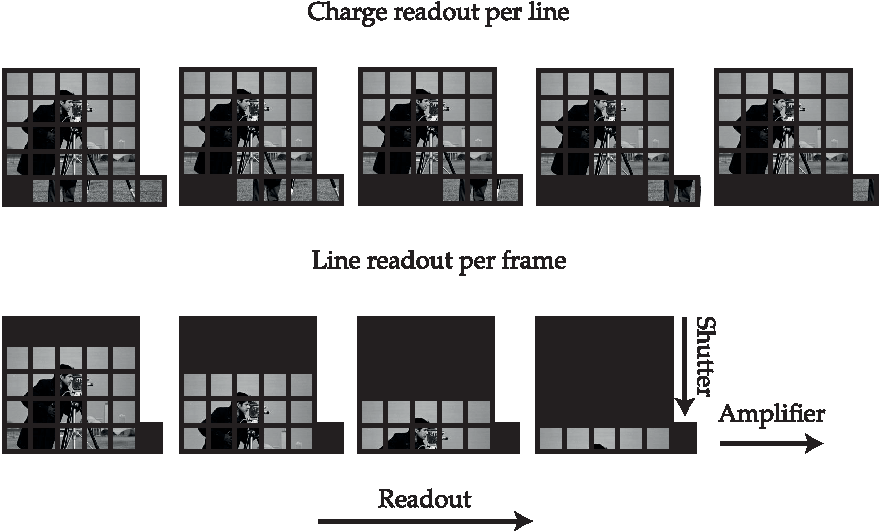
\includegraphics{./sensor_chips}
    \caption[Schematic of how electronic charge is transferred from a \gls{CCD} array through an amplifier]{Schematic of how electronic charge is transferred from a \gls{CCD} array through an amplifier.
    \textbf{Charge readout per line:} charge is serially transferred along the line being read into a single amplifier.
    \textbf{Line readout per frame:} once the line is read, the entire frame is shifted down to be read, acting as a shutter.
    Serial reading through a single amplifier is slow.}\label{fig:sensor_chips}
\end{figure}


% \begin{figure}
%     \centering
%     
\includegraphics{./imaging_sensors.pdf}
%     \caption{Imaging sensors}
%     \label{fig:imaging_sensors}
% \end{figure}

\subsection{Limits of fluorescence microscopy}

\subsubsection{Photobleaching}

Fluorescently stained samples will slowly fade in radiance (under fixed illumination) over time as the dye molecules are photochemically destroyed through photobleaching.
The process occurs typically through photo-oxidation, once the \gls{fluorophore} is in an excited state it may then energetically fall into a triplet state where it is more likely to permanently bond with oxygen radicals.
Dye medium can be buffered with scavengers of oxygen radicals to mitigate the process of bleaching.
In some \emph{in vivo} experiments, genetically modified organisms suffer less from photobleaching as molecules that have photo-bleached are continually replaced by newly expressed (transcribed) \gls{fluorophore}s.

%Whilst this is true I feel like the firsat half of the sentence is jarring.
% When imaging live samples expressing fluorescent proteins photobleached molecules can be replaced by newly transcribed(?) fluorescent proteins

\Gls{photobleaching} can be exploited to learn about a specimen, using \gls{FRAP}; wherein an imaging region is purposefully bleached, so that the rate of diffusion of unbleached dye molecules into the \gls{FOV} can be estimate.
The rate of return of intensity in the imaging region then gives a measure of diffusion.

% FRET STORM PALM
%Some molecules have the valuable property of being able to reverse

%\paragraph{Reversible photobleaching}
\subsubsection{Phototoxicity}

Fluorescent dyes can act as \gls{photosensitier} during live imaging, resulting in damage to functionality of the cell.
%What about other autofluorescent molecules in the sample and other absorbances? I think you need to mention this as one of the niches of light sheet is that it reduces light does, so make it clear just how bad too much light is
Chromophores of fluorescent proteins are shielded by direct contact from molecular oxygen through protein moiety, and so fluorescent proteins may be less phototoxic to living specimens~\cite{pawleyHandbookBiologicalConfocal2006}.
% It has beeen suggested that acceptable levels of light exposure will be on the order of a solar.
%Direct and intense light exposure


%Photodynamic effwect
%Intensity induced
%\subsection{Resolution}
\section{Three dimensional fluorescence microscopy}

The light microscope as discussed is inadequate for imaging thick three dimensional samples as light from the sample, above and below the focal plane, contributes to the detected light.

\subsection{Confocal microscopy}

Marvin Minsky proposed the first \gls{confocal microscope} in the late 1950s to image deep into brain tissue.
A pinhole is placed in a conjugate image plane in the detection path which precludes out-of-focus light from being detected.
The narrower the pinhole the better the optical sectioning, though sacrificing the received signal.

In Minsky's microscope the sample was mechanically scanned to build a volumetric image.
By mechanical scanning, the imaging speed is greatly reduced due to the speed of responses of the stage, the maximum speed of travel of the stage and the relaxation time of the stage.
Specimens are prone to spatial shifts during scanning as well, which causes distortions in the final image.

Modern \gls{confocal microscope}s use often \gls{galvanometric scanning mirrors} to sweep a laser beam through the sample to build an image.
Though faster than mechanical scanning, video-rate scanning confocal microscopy is only viable using \gls{resonant scanning mirrors} and high power lasers (due to the photon rejecting nature of the confocal pinhole).

% \subsubsection{Spinning disk confocal microscopy}
%
% The speed of Single point confocal microscopy can be greatly improved by producing multiple points.

%\subsubsection{Principles}
%\paragraph{Spinning disk confocal microscopy}
\subsection{Two photon (2P) microscopy}\label{sec:2p}

% 2P microscopy is a part of a breed of techniques called non-linear microscopes which exploit the quantum nature of fluorophores.
% 2P imaging provides the most efficient signal generation.

The photon rejecting pin-hole of \gls{confocal microscope}s can be entirely avoided by using infra-red laser sources.
Exciting a \gls{fluorophore} to an excited state requires a quantised amount of energy, which is typically supplied by a single photon.
However, two photons, each with double the desired wavelength, also contain the requisite amount of energy to cause the same excitation.
For this event to occur, there needs to be a high photon density surrounding the \gls{fluorophore}.
In a laser scanning system, this means that the beam focus of the \gls{objective lens} is the most likely place for fluorescence to occur, with a sharp decline in intensity axially, providing optical sectioning.

By using \gls{2P} excitation, greater depth imaging (\SI{\sim6}{fold} deeper) can be achieved with reduced \gls{photo-toxicity}, making the technique very useful for non-invasive live imaging.

\subsubsection{Drawbacks} %500nm -> 10^-01.4 10^+1.8

Water, which is abundant in biological specimens, has a large absorbance in the infrared spectrum, 3 orders of magnitude larger than in the visible spectrum (e.g. \SI{532}{\nano\meter} versus \SI{1064}{\nano\meter});
combined with the high energy needed to create the \gls{2P} effect at the focal point, this can cause localised heating which can in-turn be damaging to specimens and cause optical \gls{aberration}s.
Localised heating can be mitigated by moving the beam sufficiently quickly such that significant heating does not occur.
Using infrared excitation also means that the \gls{2P} imaging has a coarser lateral resolution when compared to visible confocal microscopy due to their wavelength (Equation~\eqref{eq:lateral_res}).
Finally, infrared-red laser sources are more difficult to work with for alignment than visible \gls{Laser}s.
% prohibitively expensive and, until recently, reliable turn-key solutions were not viable.

\subsection{Structured illumination microscopy}\label{sec:SIM_theory}

In \gls{SIM}, the sample is sequentially illuminated with several periodic patterns using a fast \gls{wide-field} microscope.
The mixing of each illumination pattern with the structure of the fluorescent sample results in several diffraction limited images from which a high-resolution image of the original sample can be computationally reconstructed.
Furthermore optical sectioning can also be achieved using specific illumination.
% means that additional resolution can be extracted both in \(xy \) and \(z \).

\begin{figure}
    \centering
    % \hfill
    \begin{subfigure}[t]{0.25\textwidth}
        \centering
        
\includegraphics[height=3cm]{./sim/otf}
        \caption{\Gls{wide-field} \gls{OTF}}\label{fig:sim_otf}
    \end{subfigure}\hfill
    \begin{subfigure}[t]{0.25\textwidth}
        \centering
        
\includegraphics[height=3cm]{./sim/third_flower}
        \caption{\gls{SIM} image reconstructed for one orientation with a \gls{super-resolution} improvement in \(k_y \)}\label{fig:sim_third_flower}
    \end{subfigure}\hfill
    \begin{subfigure}[t]{0.35\textwidth}
        \centering
        
\includegraphics[height=3cm]{./sim/full_flower_alt}
        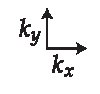
\includegraphics{./sim/xy_coordinates}%\label{fig:sim_coordinates}
        \caption{\gls{SIM} image reconstructed for three orientations, near homogenous 2D \gls{super-resolution} improvement}\label{fig:sim_full_flower}
    \end{subfigure}
    % \begin{subfigure}[t]{0.11\textwidth}
    %     \centering
    %     % \caption{Sim full flower}
    % \end{subfigure}
    % \hfill
    \caption[Schematic of \gls{SIM} reconustruction in Fourier space]
        {Schematic of \gls{SIM} reconustruction in Fourier space.
        In (\subref{fig:sim_otf}), the circular area corresponds to the passband of the \gls{objective lens}, the edge being the frequency cut-off.
        The raw data in (\subref{fig:sim_otf}) consists of superposed original image information
        positioned at three different origins.
        Once delineated, the high-resolution information can be relocated to the correct position, resulting in a wider pass-band, (\subref{fig:sim_third_flower}).
        The process is repeated three times to isotropically fill the available frequency space by rotating the illumination patterns, (\subref{fig:sim_full_flower}).
        }\label{fig:sim_flowers}
\end{figure}

As discussed in Section~\ref{sec:resolution}, an \gls{objective lens} acts as a band pass filter for low-frequency information.
From the \emph{\Gls{convolution theorem}} (see Appendix~\ref{appendix:convolution_theorem}):
\begin{align}
  \mathcal{F} (f(\mathbf{r}) \cdot g(\mathbf{r})) = \mathcal{F}(f(\mathbf{r})) * \mathcal{F}(g(\mathbf{r}))
\end{align}
% the multiplication of two signals in real-space is the convolution of the two \gls{Fourier transform}ed signals in frequency space and,
Furthermore, the convolution of two signals in real space is the multiplication of the Fourier transformed signals in frequency space.
This indicates that projecting a sinusoidal pattern in real space will convolve the Fourier transform of the sample signal in frequency space with the Fourier transform of the sinusoid signal.
The Fourier transform of a sinusoid is three delta functions at \SI{-1}, \SI{0} and \SI{+1} with a separation governed by the pattern frequency: \(k_1 = {2\pi}{\lambda} \).
And so, before the imaging system can band-pass the signal, the illumination pattern has forced three copies of the Fourier transform of the original structure into the pass band.
These copies are shifted by the vectors \(k_1 \) and \(k_{-1} \) such that high frequency information outside of the pass band of a uniformly illuminated system is now captured. %has been cumulated.
The overlaid information can then be computationally unmixed by imaging with three different sinusoidal illumination phases to delineate the \SI{-1}{}, \SI{0}{} and \SI{+1}{} orders for reconstruction, see \figurename~\ref{fig:sim_flowers}.

\subsubsection{Optical sectioning \gls{SIM}}

Three dimensional information can be extracted by manipulating frequency space even further.
For instance, the \emph{\gls{missing cone}} of axial spatial frequencies for the structures's Fourier transform (see \figurename~\ref{fig:sim_axial}) can be filled in by using an illumination pattern with \(k \)-vectors half the maximum available.
In frequency space this pushes the region of the missing cone into axial resolution maxima of the \gls{OTF} support (toroidal), giving three dimensional structure.
By adding a third beam along the optical axis to interfere with the sinusoidal pattern, a further axial sinusoidal pattern can be created.

\begin{figure}
    \centering
    \begin{subfigure}[t]{0.48\textwidth}
        \centering
        
\includegraphics[width=1\linewidth]{./sim/axial_otf}
        \caption{Widefield OTF support}\label{fig:sim_axial_otf}
    \end{subfigure}\hfill
    \begin{subfigure}[t]{0.48\textwidth}
        \centering
        
\includegraphics[width=1\linewidth]{./sim/axial_2_beam_2d}
        \caption{2-beam SIM at \SI{2}{\times}\(k_0\)\\
        2D reconstruction}\label{fig:sim_axial_2_beam_2d}
    \end{subfigure}
    \begin{subfigure}[t]{0.48\textwidth}
        \centering
        
\includegraphics[width=\linewidth]{./sim/axial_2_beam_3d}
        \caption{2-beam SIM at \SI{1.5}{\times}\(k_0\)\\
        3D reconstruction}\label{fig:sim_axial_2_beam_3d}
    \end{subfigure}
    \begin{subfigure}[t]{0.48\textwidth}
        \centering
        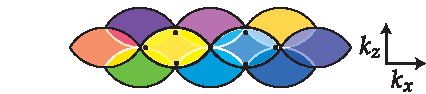
\includegraphics[width=\linewidth]{./sim/axial_3_beam}
        \caption{3-beam SIM at \SI{2}{\times}\(k_0\)\\
        3D reconstruction}\label{fig:sim_axial_3_beam}
    \end{subfigure}\hfill
    \caption[Axial view of 2 and 3 beam illumination in \gls{SIM}]{
    Axial view of 2 and 3 beam illumination in \gls{SIM}.
    Black points in (\subref{fig:sim_axial_otf}) represent lateral frequency mixing from 2-beam illumination, the grey points represent axial frequency mixing from 3-beam illumination.
    (\subref{fig:sim_axial_otf}) shows the lateral extent of 2-beam \gls{SIM} at maximum (\SI{2}{\times}) excitation frequency, with no added axial resolution.
    (\subref{fig:sim_axial_2_beam_3d}) shows the lateral extent of 2-beam \gls{SIM} at (\SI{1.5}{\times}\(k_0\)), giving reduced resolution but providing increased axial resolution.
     (\subref{fig:sim_axial_2_beam_3d}) shows the lateral and axial extent of 3-beam \gls{SIM}, doubling in resolution axially and laterally~\cite{gustafssonSurpassingLateralResolution2000}.
     The thick black outlines show the original OTF support of the widefield image.
    % Resulting OTF in (a, c) two- and (b, d) three-beam illumination. The black spots in
    % the microscope’s widefield OTFs (a: two-beam and b: three-beam) show the origins of the
    % shifted object information copies.When these copies are shifted back (c, d) to their correct
    % positions, the effective OTF increases in size. The black outline shows the original widefield
    % OTF cut-off border. The borders of the shifted OTFs are shown in gray. The corresponding
    % illumination patterns are shown in Figure 9.2a,b
    }\label{fig:sim_axial}
\end{figure}

\subsubsection{\gls{mSIM}}\label{sec:msim}

Schroff~\emph{et.~al.} showed that three dimensional, super-resolved, information can be also be extracted by \gls{mSIM}~\cite{yorkResolutionDoublingLive2012}.
\gls{mSIM} uses a square lattice of illumination points which raster scan across the sample to provide a fast, parallelised, confocal-like image.
Each spot is computationally pin-holed, and the resulting images are summed to produce a final, super-resolved image, as in \figurename~\ref{fig:mSIM}.

\begin{figure}
  \centering
  \begin{subfigure}[t]{0.185\textwidth}
    \centering
    \includegraphics[width=\linewidth]{msim/raw_excited}
    \caption{A lattice of illumination points}\label{fig:msim/raw_excited}
  \end{subfigure}\hfill
  \begin{subfigure}[t]{0.185\textwidth}
    \centering
    \includegraphics[width=\linewidth]{msim/recorded_excited}
    \caption{The image as recorded by the detector}\label{fig:msim/recorded_excited}
  \end{subfigure}\hfill
  \begin{subfigure}[t]{0.185\textwidth}
    \centering
    \includegraphics[width=\textwidth]{msim/digital_pinholing}
    \caption{Digital pin-holing}\label{fig:msim/digital_pinholing}
  \end{subfigure}\hfill
  \begin{subfigure}[t]{0.185\textwidth}
    \centering
    \includegraphics[width=\linewidth]{msim/column}
    \caption{Reconstructing}\label{fig:msim/column}
  \end{subfigure}\hfill
  \begin{subfigure}[t]{0.185\textwidth}
    \centering
    \includegraphics[width=\linewidth]{msim/reconstructed}
    \caption{Full mSIM reconstruction}\label{fig:msim/reconstructed}
  \end{subfigure} % \includegraphics{/path/to/figure}
  \caption[Schematic of \gls{mSIM} reconstruction]{
  Schematic of \gls{mSIM} reconstruction. \gls{mSIM} uses a square lattice of illumination spots in (a) and (b); which are digitally pin-holed in (c); and raster scanned in (d); to build a super-resolved image in (e)}\label{fig:mSIM}
\end{figure}

% After separation, the information can be shifted back to
% its respective position, resulting in an expanded accessible frequency area (c). To expand
% the resolution in the object plane not only along one direction but also isotropically,
% the illumination pattern is subsequently rotated to carry out the image acquisition with
% several illumination pattern orientations (d).}

% \subsubsection{Drawbacks}

\subsection{Selective plane illumination microscopy}

The techniques as introduced above all provide volumetric imaging through reconstruction.
Structured illumination techniques require computation reconstruction which is prone to artefacts.
Confocal scanning is slow and generally lossy with signal.
Light-sheet microscopy offers reconstruction-free, fast, low photo-toxicity volumetric imaging.
The application of light-sheet microscopy is the focus of this thesis and will be introduced in detail in the following chapter.

% In light sheet microscopy, the sample is illuminated with a thin sheet of light to obtain optical sections.
% The microscope generally consists of two orthogonal optical axes: one for generating the light sheet for illumination, and the other for widefield detection of the emitted fluorescence.
% The two axes are aligned such that the illuminating light sheet is positioned in the focal plane of the detection unit.
% As the specimen is illuminated with a sheet of light, the entire focal plane of the detection arm is illuminated providing instant optical sectioning as opposed to the slow point scanning used in confocal microscopy (Chapter 5).
